\section{paper reading}
\subsection{background}

The volume rendering process requires some concepts as followed:

For each ray start at $\mathbf{0}$ and on the direction $\mathbf{d}$, the ray $\mathbf{r}$ could be described as $\mathbf{r}(t) = \mathbf{o} + t\mathbf{d}$.

For each point $x$, the color of it is represented as $c(\mathbf{x})=c(\mathbf{r}(t))=c(t)$.

The occupation a.k.a. the volume density is the probability that the ray hit a particle at the position $\mathbf{x}$ is represented as $\sigma(\mathbf{x})=\sigma(\mathbf{r}(t))=\sigma(t)$.

The transmittance is the probability of a ray travelling from time $0$ to time $t$ without hitting any particles, and it is represented as $T(t)=\exp(-\int_{0}^{t}\sigma(t)dt)$.

So the expectation of the color that the ray $\mathbf{r}$ throw volume rendering is that:
\begin{equation}
C(\mathbf{r}) = \int_{t_n}^{t_f} T(t)\sigma(t)\mathbf{c}(\mathbf{r}(t),\mathbf{d})dt + T(t_f)C_{bg}
\label{volumn rending}
\end{equation}
Where $C_{bg}$ is considered as the color of the background, usually take $(0,0,0)^{\top}$ or $(1,1,1)^{\top}$.

\begin{figure}[htbp]
\centering
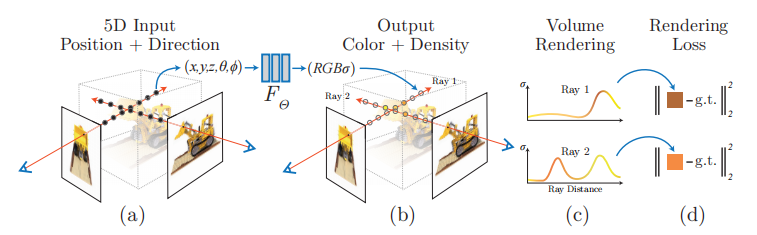
\includegraphics[width=0.9\linewidth]{img/NeRF.png}
\caption{pipeline of NeRF}
\label{NeRF pipeline}
\end{figure}

The NeRF's pipeline could be seen in figure \ref{NeRF pipeline}. With the formula of volume rendering formula \ref{volumn rending}, we could train the network using the trained implicit function $F_{\Theta}$, with input $(x,y,z,\theta,\phi)$, then output the $(R,G,B,\sigma)$ for the correspondence input, where $\sigma$ is the volume density.

With the volume rending formula \ref{volumn rending}, we could computer the image with given $(x,y,z,\theta,\phi)$. Then we can compute the rendering loss \ref{nerf loss}, in order to train a implicit model $F_{\Theta}$ for a certain scenario.

The loss function is defined as:
\begin{equation}
\mathcal{L}=\sum_{\mathbf{r}\in\mathcal{R}}\big[\|\hat{C}_c(\mathbf{r})-C(\mathbf{r})\|_2^2-\|\hat{C}_f(\mathbf{r})-C(\mathbf{r})\|_2^2\big]
\label{nerf loss}
\end{equation}

The NeRF method also takes some tricks to improve the performance, such as the positional encoding 
$$\gamma(p)=(\sin(2^0\pi p),(\cos(2^0\pi p),\cdots,(\sin(2^{L-1}\pi p),(\cos(2^{L-1}\pi p))$$

But the vanilla NeRF has some problem and trained slowly, so the TensoRF \ref{TensoRF paper reading} and Instant-NGP \ref{instant ngp paper reading} and etc. methods were proposed.

% --------------------------------
\subsection{TensoRF}
\label{TensoRF paper reading}

\begin{figure}[htbp]
\centering
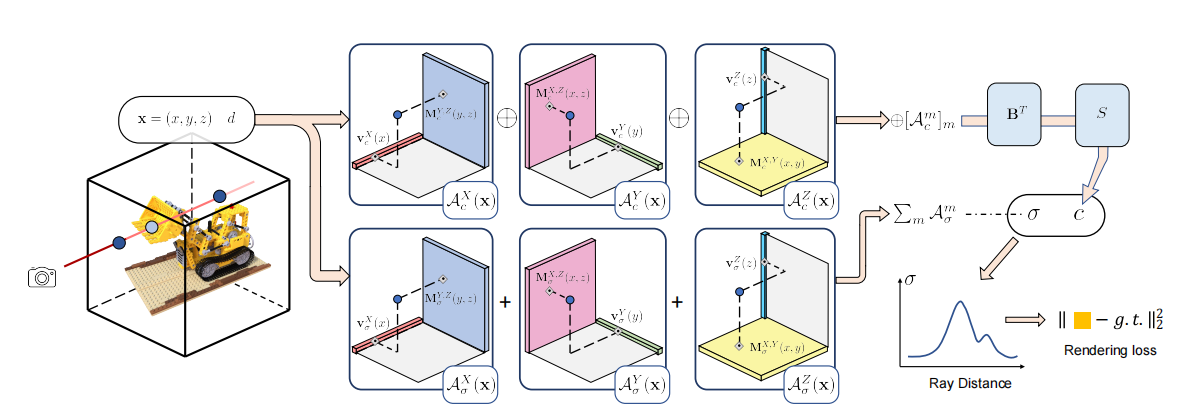
\includegraphics[width=0.9\linewidth]{img/TensoRF.png}
\caption{pipeline of TensoRF}
\label{TensoRF pipeline}
\end{figure}

The work TensoRF(Tensorial Radiance Fields) \cite{TensoRF} proposed a fast training method that does not require a large amount of storage space, comparable to SOTA in rendering quality.

The pipeline of TensoRF could be seen in figure \ref{TensoRF pipeline}.

The vanilla NeRF is based on the coordinates, which uses voxel grid. This requires a large GPU memory to store them, increase in the space complexity of $O(n^3)$, $n$ is the scenario's size.

The key idea is to use a Vector Matrix (VM) decomposition algorithm. Using fewer component tensors to represent a scene and rendering images faster and better. The vanilla NeRF did not effectively use the voxel grid, so each feature grid could be seen as a $4$ dimension tensor. The first $3$ dimension is the space coordinate $x,y,z$, and the $4$-th dimension is the feature. Then the decomposition algorithm could be used greatly reduced to memory consumption. And it has universality and can be innovated using various tensor decomposition algorithms.

The pipeline figure \ref{TensoRF pipeline} shows that the neural radiance field expressed as a set of vectors $v$ and matrix $M$, calculate the volume density and color from this. For each spatial coordinate, we use linear or bilinear sampled values to simulate trilinear interpolation. Add up the volume density along the rays to obtain a density value of $A_{\sigma}$. Stack the color values together to obtain a vector, then multiply it with the appearance matrix $B$, and use the decoding function $S$ to obtain the color $c$.

So we can see that the TensoRF could greatly improve the training efficiency of of the NeRF's process. 

% --------------------------------
\subsection{Instant-NGP}
\label{instant ngp paper reading}

\begin{figure}[htbp]
\centering
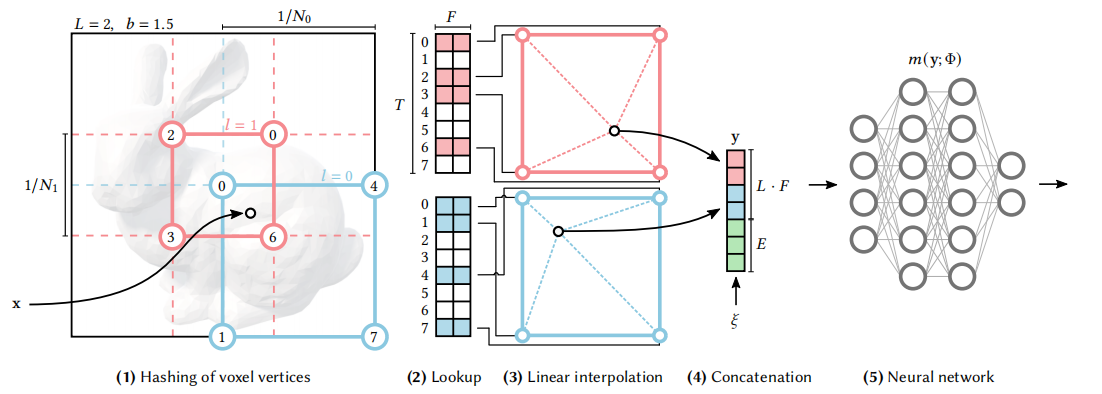
\includegraphics[width=0.9\linewidth]{img/hash_encoder.png}
\caption{hash encoder}
\label{hash encoder}
\end{figure}

The work Instant-NGP(Instant Neural Graphics Primitives) \cite{instant-ngp} proposed a way that with hash encoding in figure \ref{hash encoder}. It firstly converts the coordinate $(x,y,z)$ into the index of the hash table. And the different resolution level has different results(red and blue in the figure). Then do the tri-linear interpolation, concat the result vectors as the feature vector. Then the feature vector is sent to the neural network. 

The Instant-NGP mainly used $2$ MLP, one is similar to the vanilla NeRF,  the density feature encoding at multiple resolutions corresponding to the sampling point is output by the multi solution hash encoding, mixed according to different weights, and decoded to obtain the true density value.

Compared dimensions of MLP in NGP and the number of layers in the network is also much smaller than the vanilla NeRF. This makes Instant-NGP run much faster than the vinalla NeRF.

% --------------------------------
\subsection{Nerfstudio}
The work Nerfstudio \cite{nerfstudio} proposed an integration work, it integrate various NeRF technologies into reusable modular components. And it did real time visualization of NeRF scenes through rich controls. Which makes users much easier to use the tools and the pipeline.